
Over the code analysis and modelization of the \textit{DBT} component, the bindings and interfaces established with the Decoder became evident. By inspection, it is possible to see that this component has an interface with the following components: Source Architecture, Source Environment, CCache, Generator and Translator. Next, each binding will be covered one-by-one, being revealed its importance as well as the methods that composes it.

\subsubsection*{Decoder - Source Architecture}
    The Source Architecture is the component that only provides services. The reason for that is based on the fact that its essence consists in the specification of the contents of an architecture. Figure \ref{fig:DecoderBind1}, there are \textbf{two interfaces} between the Decoder and the Source Architecture components (figure \ref{fig:DecoderBind1}).
    
    \begin{figure}[!htb]
    \centerline{
    \includegraphics[scale=0.45]{images/DecoderBind1}
    }
    \caption{Decoder - Source Architecture bindings.}
    \label{fig:DecoderBind1} 
    \end{figure}
    
    The first binding (\textbf{R4\_1 - S4}) lies in an interface which has a function that returns the number of bits of the opcode (\texttt{nBitsOpcode}). This value is used in the generation of the final sources by the elaboration files. In the second binding (\textbf{R6\_1 - S6}), the interface \texttt{Registers} is recognized as an empty interface, \textit{i.e.}, exists and must be respected but there is no way of define functions on it because each architecture has its own registers. In the source files, the definitions of the registers is found in an header file as macros.


\subsubsection*{Decoder - Source Environment}
    As the name suggests, the Source Environment is associated to important elements of the execution environment such as the \textit{PC} and the data memory. 
    
    \begin{figure}[!htb]
    \centerline{
    \includegraphics[scale=0.45]{images/DecoderBind2}
    }
    \caption{Decoder - Source Environment binding.}
    \label{fig:DecoderBind2} 
    \end{figure}
    
    For the Decoder, the value stored \textit{PC} is necessary in decoding branch instructions. Thereby, one of the services that the Source Environment component must provide is the \textit{PC} access which translates in to an interface whose methods must allow get and set the \textit{PC} value, \texttt{getPC} and \texttt{setPC} (figure \ref{fig:DecoderBind2}). 
     
    \subsubsection*{Decoder - CCache}
    In order to decode the operands of an instruction, it is necessary in a prime instance to fetch it. This step is made inside the decoder since the length of the instruction depends of the source ISA, and so, there are situation where this value is not constant. For those situation, the instructions must be fist detected and after fetched. Figure \ref{fig:DecoderBind3} shows the binding established.
    
    \begin{figure}[!htb]
    \centerline{
    \includegraphics[scale=0.45]{images/DecoderBind3}
    }
    \caption{Decoder - CCcache binding.}
    \label{fig:DecoderBind3} 
    \end{figure}
    
    As has been said before, CCache stores portions of binary source code that needs to be translated. Thus, an interface is established and must contain a function that accesses the memory and returns an instruction (\texttt{fetch}). 
       
    \subsubsection*{Decoder - Generator}
    
    Among other responsibilities, the decoder decides which methods must be called for target code generation. This generation service is provided by the Generator which contains the implementations of the generation functions for the target architecture.
	That being said, an interface between the Decoder and the Generator is visible and consists in the \texttt{gen\_x} functions that were mentioned before. Examples of \texttt{gen\_x} functions are shown in figure \ref{fig:DecoderBind4}.
    
    \begin{figure}[!htb]
    \centerline{
    \includegraphics[scale=0.45]{images/DecoderBind4}
    }
    \caption{Decoder - Generator binding.}
    \label{fig:DecoderBind4} 
    \end{figure}
    
    
\subsubsection*{Decoder - DBT Engine}   
    The last service referenced by the Decoder is provided by the DBT Engine (figure \ref{fig:DecoderBind6}). It is composed internal variables of the engine, such as, \texttt{eoBB} (signals the end of a basic block, and so, the end of translation), \texttt{eoExec} (signals the end of execution) and at last \texttt{pSourceProgMem} (pointer to code memory used in instructions that access this the contents of it).
    
	\begin{figure}[!htb]
    \centerline{
    \includegraphics[scale=0.45]{images/DecodeBind6}
    }
    \caption{Decoder - DBT Engine binding.}
    \label{fig:DecoderBind6} 
    \end{figure}
    

\subsubsection*{Decoder - Translator}

	Until now, all the bindings of the Decoder were references to services of other components. But, concerning the correct operation of the DBT engine, the decoder must step in and provide a decoding service to the translator (figure \ref{fig:DecoderBind5}).
    
	\begin{figure}[!htb]
    \centerline{
    \includegraphics[scale=0.45]{images/DecoderBinding5}
    }
    \caption{Decoder - Translator binding.}
    \label{fig:DecoderBind5} 
    \end{figure}
    
    A connection between the Decoder and the Translator is established, consisting in an interface that contains a \texttt{decode} function. So, when a dynamic binary translator is created using the reference architecture that is being design, an implementation of a decode function must inevitably exist.

%%%%%%%%%%%%%
% Decoder Behaviors
%%%%%%%%%%%%%%
\subsection{Decoder Behaviors}

As mentioned, decoding the operands of the source instructions for target code generation can be performed in several ways, therefore, this sections presents some behaviors associated with different implementations (software and hardware approaches). This is done since the EL language allows to define non-final components. This means that, for each behavior, an elaboration file must be created and the source files associated must be annotated accordingly. At the end, the user can select the desired elaboration for this component among the many implemented and theirs specific properties that are specific for the implementation and not referenced in the model.


\subsubsection{Switch Cases}
    This kind of decoder behavior is presented in the original \textit{DBT}, the one that is served as a base to the designed reference architecture. Figure \ref{fig:Decoders_Behavior1} shows the decoder's behavior workflow.

    \begin{figure}[!htb]
        \centerline{
        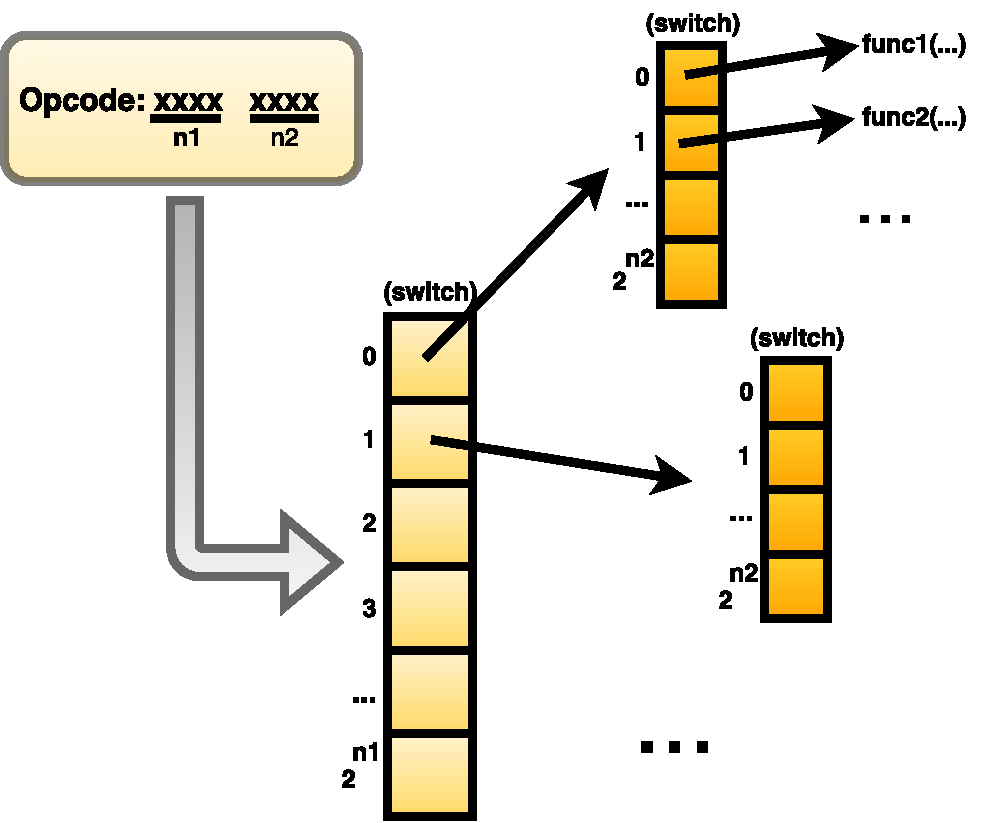
\includegraphics[scale=0.5]{images/Decoders_Behavior1}
        }
        \caption{Decoder's Switch Cases behavior.}
        \label{fig:Decoders_Behavior1} 
        \end{figure}
    
     As the name suggests, the principle operation is based on switch cases which can be only one or several. By so, it follows a simple proposal of a decoder which presents a straightforward operation strategy. It will be seen that it may carry \textbf{some overhead} which can be easily reduced. The opcode is useful because it serves as a guider during the travel along the switch cases. The technique can be described in this 3 steps:
    
    \begin{enumerate}
    
   		\item The opcode is acquired and split. The number of splits will define the number of branches that will occur.
        
        \item It is relevant to know the number of bits of the opcode as well as the number of bits that each portion. Having those values (represented in figure \ref{fig:Decoders_Behavior1} as \textbf{N1} and \textbf{N2}), the size of the first switch case will be 2$^{N1}$. From there, each entry in the switch case will contain another switch case with the size of 2$^{N2}$. If there is no divisions, there will be only one switch case with the length equaling the number of instructions. N1 and N2 are specific properties configurable by the user.

		\item Finally, having the switch cases structure defined, the output is a callback function for a specif instruction. This method implements exactly the steps for decode the instruction. Thereby, given an opcode the result is, in a certain way, a jump to a function.
	\end{enumerate}
    
    To sum up, this process can introduce some overhead if only exists one switch case. This may happens since to reach the correct entry of the switch case, the traversal can be bigger for some instructions. This overhead can be reduced by creating another switch case inside. 

   
\subsubsection{Jump Table}

Between the several behaviors for the Decoder component that will be presented in this chapter, a non implemented one is based on a jump table (figure \ref{fig:Decoders_Behavior2}). A jump table (or branch table) is basically a method of transferring program control to another part of the program (loaded dynamically). There are situations where the compiler creates jump tables from optimized switch statements, however, that can not always be guaranteed. Attending the problem stated in this section, a jump tables was design as a new possible implementation for the decoder. 

Instead of using a switch case to detect the instruction and calling the corresponding generating method, an array is used as the data structure that stores callback functions, indexed with the opcode of the instruction. This behavior can easily be implemented since the callback functions are the same used in the "switch decoder". 

\begin{figure}[
H]
\centerline{
\includegraphics[scale=0.45]{images/Decoder_Behavior2}
}
\caption{Decoder's Jump Cases behavior.}
\label{fig:Decoders_Behavior2} 
\end{figure}


\subsubsection{Generic Decoder}

Another possible implementation for a decoder follows a generic one (Figure \ref{fig:Decoders_Behavior4}), that can be used for any architecture in this reference architecture.  


\begin{figure}[!htb]
\centerline{
\includegraphics[scale=0.45]{images/Decoders_Behavior4_2}
}
\caption{Decoder's Generic behavior.}
\label{fig:Decoders_Behavior4} 
\end{figure}

This type of decoder follows the same principle of a vector indexed by the opcode. However, instead of an address of a function, the vector contains a structures with information about the instruction. 

The structure in each node is composed by two tables named:
\begin{itemize}
\item \textbf{Step Table}, which stores the specific steps that must be performed since the fetch of the instruction until the generation of target code.
\item \textbf{Variable Matrix}, which stores references for variables used inside those steps. Each raw belongs to a function of the step table.
\end{itemize}

In this approach, the hard work relies in building the main table since every instruction must be analyzed and transposed into the structure.  


    \subsubsection{Instruction Format}
    For this last decode procedure, an exhausting study of the source ISA was required. That study was focused on the creation of groups according to the instructions format of 8051 (for this case of study).
    
   
    \begin{figure}[!htb]
    \centerline{
    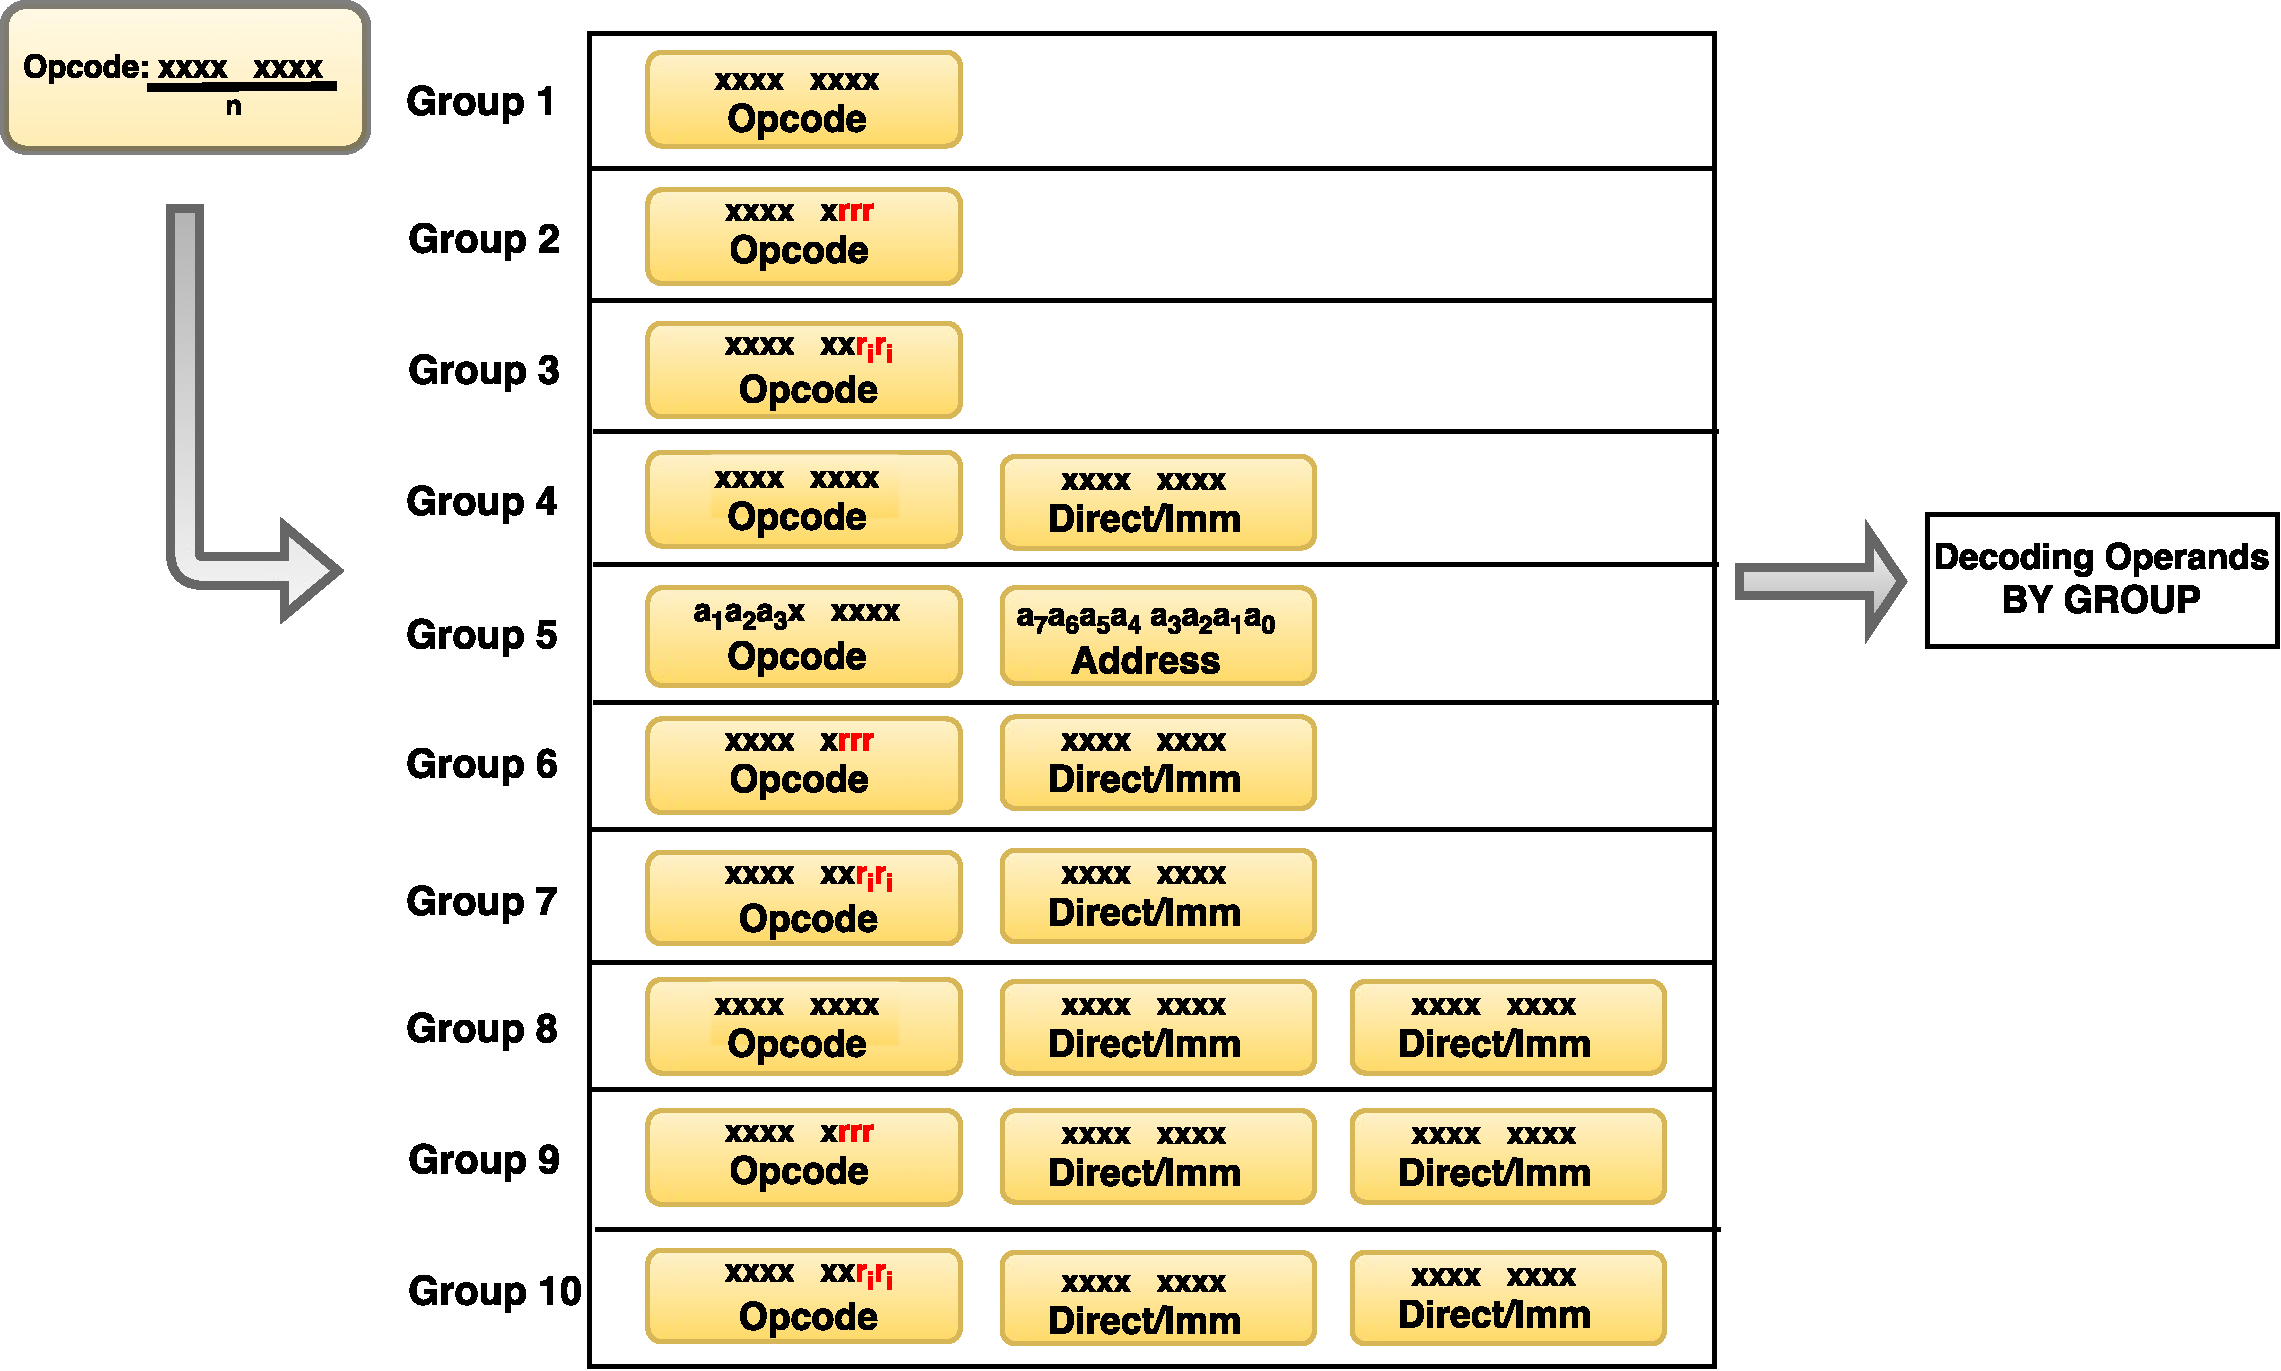
\includegraphics[scale=0.4]{images/Decoders_Behaviors3}
    }
    \caption{Decoder's Instruction Format behavior.}
    \label{fig:Decoders_Behavior3} 
    \end{figure}
	
    This type of decoder is also not implemented. Therefore, in order to achieve that gold, and since its behavior is based on the format of the instructions, there was also the need to check each instruction, evaluate it and according to its format, put it in the specif group. At the end, the result was the existence of 10 groups with the corresponding instruction format, as shown in figure \ref{fig:Decoders_Behavior3}. 
	Having the definition of the groups, the process is quite trivial. Basically, the opcode is acquired, and accordingly with its group, the operands are obtained. Due the selection of the group and other actions that must be executed, this behavior can cost a big price with a software implementation and can become a disadvantage. So, theoretically, a good alternative can be an hardware implementation. However, this implementation requires a different interface in the model (since the target instructions are created without intermediate representation using the operands obtained from the source instruction). For that, an appropriate (and additional) implementation in the generator shall be obtained to accomplish this approach. 